
% *** Authors should verify (and, if needed, correct) their LaTeX system  ***
% *** with the testflow diagnostic prior to trusting their LaTeX platform ***
% *** with production work. IEEE's font choices can trigger bugs that do  ***
% *** not appear when using other class files.                            ***
% The testflow support page is at:
% http://www.michaelshell.org/tex/testflow/

\documentclass[conference, compsoc]{IEEEtran}

\usepackage{graphicx}
\usepackage{color}
\usepackage{bussproofs} 
\usepackage{listings}
%\include{prooftree}

\usepackage{listings}
\usepackage{keyval}
\usepackage{ifthen}
\usepackage{alltt}

% alguns comandos
\newcommand{\Fix}[1]{\textbf{[[#1]]}}   
\newcommand{\truee}{\mathbf{true}}
\newtheorem{refine}{\bf{Refactoring}}
\newenvironment{refinement}[1]
   {\begin{refine} \normalfont \lawName{#1} \\ \noindent}
   {\end{refine}}
\newcommand{\bfoo}{\bfooc{true}}
\newcommand{\efoo}{\efooc{true}}
\newcommand{\bfooc}[1]
   {\ifthenelse{\equal{#1}{true}}{\begin{alltt}}{\begin{forget}}}
\newcommand{\efooc}[1]
    {\ifthenelse{\equal{#1}{true}}{\end{alltt}}{\end{forget}}}

\newcommand{\cc}[1]{\ensuremath{#1}}


       
\begin{document}

\lstset{language=Haskell, basicstyle=\small,aboveskip=10pt}


%
% paper title
% can use linebreaks \\ within to get better formatting as desired
\title{Detecting Errors and Bad Smells in Feature Modeling}


% author names and affiliations
% use a multiple column layout for up to two different
% affiliations

\author{\IEEEauthorblockN{Rodrigo Bonif\'{a}cio, Leopoldo Teixeira, Paulo Borba}
\IEEEauthorblockA{Informatics Center\\
Federal University of Pernambuco\\
Recife, Brazil\\
\{rba2,lmt,phmb\}@cin.ufpe.br}
\and
\IEEEauthorblockN{Rohit Gheyi, Tiago Massoni }
\IEEEauthorblockA{Department of Computer Science\\
Federal University of Campina Grande\\
Campina Grande, Brazil\\
\{rohit, massoni\}@dsc.ufcg.edu.br}
}

% conference papers do not typically use \thanks and this command
% is locked out in conference mode. If really needed, such as for
% the acknowledgment of grants, issue a \IEEEoverridecommandlockouts
% after \documentclass

% for over three affiliations, or if they all won't fit within the width
% of the page, use this alternative format:
% 
%\author{\IEEEauthorblockN{Michael Shell\IEEEauthorrefmark{1},
%Homer Simpson\IEEEauthorrefmark{2},
%James Kirk\IEEEauthorrefmark{3}, 
%Montgomery Scott\IEEEauthorrefmark{3} and
%Eldon Tyrell\IEEEauthorrefmark{4}}
%\IEEEauthorblockA{\IEEEauthorrefmark{1}School of Electrical and Computer Engineering\\
%Georgia Institute of Technology,
%Atlanta, Georgia 30332--0250\\ Email: see http://www.michaelshell.org/contact.html}
%\IEEEauthorblockA{\IEEEauthorrefmark{2}Twentieth Century Fox, Springfield, USA\\
%Email: homer@thesimpsons.com}
%\IEEEauthorblockA{\IEEEauthorrefmark{3}Starfleet Academy, San Francisco, California 96678-2391\\
%Telephone: (800) 555--1212, Fax: (888) 555--1212}
%\IEEEauthorblockA{\IEEEauthorrefmark{4}Tyrell Inc., 123 Replicant Street, Los Angeles, California 90210--4321}}


% make the title area
\maketitle


\begin{abstract}
% contexto
Feature modeling is a worth and widespread approach for 
representing the common and variant capabilities of a software 
product line. 
% problema
However, besides the recent proposals for feature model semantics, 
there is a lack of definition regarding the characteristics of a 
well typed feature model. Moreover, even being well typed, models
may be badly structured. There are no catalog of bad smells for feature models
in order to help domain analysts. 
% solu��o
In this paper, we go a step further in this direction, formalizing 
typing rules and bad smells for feature modeling and presenting 
an automated approach for revealing these problems. Moreover, we propose
FM refactorings for removing the bad smells.
% avalia��o
%Our proposal 
%approach efficiently reveals type errors and bad-smells in models with 
% acho que no m�nimo temos que avaliar em 5000 diante dos papers atuais
%at most 5000 features. 
% aplica��o
This formalization can be useful for showing that FM transformations, such as
refactorings, do not introduce type errors.
% colocar mais aplica��es
\end{abstract}

\section{Introduction}
\label{sec:intro}

% contexto
Feature modeling is a well known technique for 
representing the concepts of a software domain. In fact, 
systematic reuse and domain driven approaches, such 
as Software Product Line~\cite{Clements:2001aa,Pohl:2005aa}, 
Generative Programming~\cite{Czarnecki:2000aa}, and Software 
Factories~\cite{Greenfield:2003aa}, rely on some kind of feature based notation. 
% problema
However, despite the recent proposals for defining the semantics~\cite{Schobbens:2007aa} and for reasoning 
about feature models, there is still a lack of definitions regarding \emph{type-checking} 
and \emph{well-formedness rules} of feature models. Even being well typed, a feature model may
be badly structured. Similar to programs~\cite{Fowler:1999aa}, there are a number of symptoms,
also known as bad smells, that can be useful for identifying them.

%\Fix{Rohit: eu ainda acho que ser satisfativel nao e uma regra de tipo, e sim tem haver com a semantica. Pelos papers que li, nao vi nada falando sobre regras de boa formacao e do sistema de tipos para FMs.o sistema de tipos, nos fizemos mas era bem simples. Acho que as regras de boa formacao sao as mais complicadads de definir (especialmente a completude delas).}
%\Fix{Rodrigo: beleza Rohit. Entao esse eh mais um diferencial do trabalho nosso trabalho em relacao as propostas de Benavides, certo? Ou seja, ele considera um feature model valido quando aceita pelo menos uma instancia. A nossa visao eh diferente, talvez mais ampla...certo? Seria interessante deixar isso mais claro no proximo paragrado.}

%For instance, Benavides and others argue that a feature model is valid if exists at least 
%one selection of features that satisfies the feature model constraints~\cite{Benavides:2005aa}. 
%Although we agree that such a constraint must be satisfied, we have to check other properties 
%in order to assume a feature model as being well typed. For example, according to their point 
%of view, the feature model of Figure~\ref{fig:fm01} would be considered well typed--- actually, there are several 
%valid configurations for this feature model. 

%\Fix{Rohit: Na verdade, acho que eles nao se preocuparam com a boa tipagem. Acredito que eles tenham assumido isso como hipotese do trabalho. Este comentario e o outro foram mais questao de como contar a historia e nao questionando a contribuicao. O exemplo motivante e muito bom. Seria bem interessante se encontrassemos um erro mais complicado e dificil de ver. Talvez a aplicacao de refatoramentos (ver aplicacoes de Rodrigo ou nossas de refatoramentos) pode levar a erros de boa formacao, e nao como um modelo unico.}

%However, we cannot assume the constraint $C\ \Rightarrow\ E$ as 
%being well typed, since it makes references to the a feature (E) that does not exist in the feature model. 
%This problem, which might be motivated by a typographical error, would result in a 
%feature model with a missing constraint. For larger and evolving feature models, 
%checking for these types of errors is mandatory. 

% motivacao no exemplo sobre sistema de tipos
Figure~\ref{fig:fm01} depicts a feature model. To our knowledge there is no formal definition stating what
are the properties that a well typed model must have. This may be useful, for instance, when proposing
feature model transformations. A transformation must transform a well typed model into another well typed
model. It is undesired to introduce type errors. 
% motivacao no exemplo sobre bad smells
When modeling feature models with hundreds of features, its structure may start to degrade.
For example, in the feature model depicted in Figure~\ref{fig:fm01}, notice that 
the mandatory feature B implies the optional feature D. Defining such a kind of constraint 
may be suspicious, since it is similar to changing the cardinality of feature D, which becomes a mandatory 
feature in the presence of this constraint. We consider this a bad design (\emph{bad smell}), and should be reported 
to the domain analyst in order to improve (\emph{refactor}) the underline feature model. 

\begin{figure}[thb]
\begin{center}
\input{images/fm01.pstex_t} 
 \caption{Feature model sample}
 \label{fig:fm01}
\end{center}
\end{figure}

%\Fix{Rohit: seria bom detalhar mais a importancia da formalizacao no paper de AOSD.}
%\Fix{Rodrigo: achei muito interessante a visao que voce apresentou Rohit. No paper de AOSD, o modelo de features eh usado para verificar se a selecao de features que define um produto eh valida. Por outro lado, o modelo de features tem que estar bem tipado para que essa verificacao possa ocorrer. Eh issso que tenho que deixar claro nesse paragrafo, certo?}
%\Fix{Tiago: aqui estamos referenciando muito trabalhos da UFPE, acho que nao pega muito bem pros revisores, melhor aumentar}

% solucao
In this paper, we formalize a type system for feature models. Moreover, we propose a number of bad smells of feature models. Refactorings are also proposed for removing them. The formalization may be useful in some contexts. We explore two of them in Section~\ref{sec:evaluation}.
% aplicacao
% 1. formalizacao do sistema de tipos
% paper de AOSD
For instance, a type checking activity for feature models is an essential step before applying the transformations described by Bonif\'{a}cio and Borba~\cite{Bonifacio:2009aa}, although we believe that it might be also necessary to other approaches for automated product line engineering.
% refatoramentos
This formalization is also useful for proving that FM refactorings~\cite{Alves:2006aa} do not introduce type errors. So, besides showing that the resulting FM contains all configurations of the initial one, we must prove that from a well formed FM, the resulting FM is always well-formed.

% 2. bad smells
Besides exploring type errors, we explore symptoms that may suggest bad designs. Detecting bad smells is an essential practice for the reactive approach of SPL development, since it can detect recurrence faults when modeling and evolving large feature models (with thousands of features and constraints). 
% resumo
Therefore, the contributions of this paper are three-fold:
\begin{itemize}
\item formalize well-formedness rules and a type system that must be 
obeyed in order to consider a feature model well-typed (Section~\ref{sec:type-checker});
\item propose a catalog of bad smells for feature modeling, 
which can help business analysts to find out common faults when 
designing and evolving feature models (Section~\ref{sec:bad-smells}); and
\item present the tool support used for checking whether a feature model 
is well typed, for detecting bad smells and applying some refactoring for
removing them (Section~\ref{sec:tool-support}). 
\end{itemize}


%\Fix{Acho que tem que relacionar mais a contribuicao do type checking com a contribuicao dos bad smells - nao t� muito claro qual a rela��o entre eles. Por exemplo, poderiamos questionar se bad smells s� ocorrem em modelos bem ou mal tipados?}

%We also show that the proposed tool scales to XYZ features (Section~\ref{sec:evaluation}).  

%\Fix{Rodrigo: acho que a formalizacao eh melhor expressa em Alloy, alem de ganharmos um analisador de graca--- existem checkers para Haskell, mas temos que escrever algum codigo para usa-los.  Em termos de suporte ferramental, ai poderiamos pensei em estender as bibliotecas Haskell, que hoje jah possuem interface (por meio de parsers) com fmide, e fmp. Temos que decidir se eh valido ter essas duas visoes no paper, ou usar apenas Alloy. Caso apresentemos um suporte ferramental alem do analisador Alloy, teriamos que ver como encaixar e justificar. Em SPLC, acho que descrever um suporte ferramental pode render alguns pontos.}

%\Fix{Tiago: se usarmos Haskell, qual � a vantagem de uma abordagem funcional? mais expressividade em descrever regras de tipo? acho que desempenho n�o �...}

%Additionally, we compare our work to the body of knowledge related to feature
%model semantics, reasoning and refactoring (Section~\ref{sec:related}). Finally, 
%some concluding remarks and future work proposals are presented in 
%Section~\ref{sec:concluding}.


\section{Type System}
\label{sec:type-checker}

One of the main concerns in our research work is \emph{type safety} in feature models, in order to prevent erroneous or undesirable analysis results. We consider a feature model well-typed if a number of well-formation constraints are obeyed. We present these rules in this section, both informally and using a formalization language with conventional notation mixed with the PVS language~\cite{Owre:2009aa}. Notice that this is a minimal set of constraints, as derived from our knowledge about the requirements for verifying that a selection of features is a valid member of a feature model.

We begin by providing a formal definition for feature models, which are composed of a root feature, relations, features and formulae. While \texttt{Feature} is an uninterpreted type -- with a name -- relation is a PVS datatype with four distinct classes: optional (\texttt{OPT\_REL}), mandatory (\texttt{MAND\_REL}), alternative (\texttt{ALT\_REL}) and Or-feature (\texttt{OR\_REL}). While the first two types are defined between two features, the latter are defined between a parent and a set of child features. Furthermore, we consider a set of formulae for defining constraints over the feature model (in this case, core formulae only, such as negation, conjunction and implication).

\bfoo{\small
  FM: type = [# 
    root: Feature,
    relations: set[Relation]
    features: set[Feature], 
    formulae: set[Formula] 
  #]

  Relation: datatype
  begin 
  	OPT_REL(p,c: Feature):OPT?:Relation
  	MAND_REL(p,c: Feature):MAND?:Relation
  	ALT_REL(p: Feature,c:set[Feature]):
  	  ALT?:Relation
  	OR_REL(p: Feature,c:set[Feature]):
  	  OR?:Relation
	end Relation
	
	Formula : datatype
    TRUE_FORMULA:TRUE?:Formula
    FALSE_FORMULA:FALSE?:Formula
    NAME_FORMULA(n: Name):NAME?:Formula
    NOT_FORMULA(f: Formula):NOT?:Formula
    AND_FORMULA(f0,f1: Formula):
        AND?:Formula
    IMPLIES_FORMULA(f0,f1:Formula):
        IMPLIES?:Formula
  end Formula
}\efoo%

A feature model is well typed iff its feature tree is well formed and its constraints are well typed. A feature tree must satisfy the following well-formedness rules:
\begin{itemize}
	\item there must exist exactly one root feature (already contemplated in the previous \texttt{FM} definition);
	\item features must form a tree, as a connected and acyclic graph;
	\item feature names must be unique;
	\item all relations are well formed.
\end{itemize}
%{\bf (F.)} Consider $f \in F$, where F is the set of features defined in a feature tree. If $f$ is a \emph{Basic-feature}, it will always be well typed. Otherwise, if $f$ is an \emph{Or-feature} or an \emph{Alternative-feature}, $f$ will be well typed iff $children (f) \neq \emptyset$. 

\bfoo{\small
  wellTyped(fm: FM): boolean =
    wellFormednessRules(fm) \cc{\wedge} 
    wellTypedFormulae(fm)

  wellFormednessRules(fm: FM): bool = 
    tree(fm) \cc{\wedge} uniqueFeatureNames(fm) \cc{\wedge}
    wellFormedRelations(fm)

}\efoo

For the \texttt{tree} predicate, two other auxiliary predicates must be valid: all features must constitute a graph that is both \emph{acyclic} and \emph{connected}; these predicates use the \texttt{children} function, which returns the transitive closure of the set of relations within the feature model. In addition, relations are well-formed when they relate the correct number of features for the considered relation type. For instance, alternative relations must relate at least one parent and one child feature.


\bfoo{\small
  tree(fm: FM): bool = 
      acyclic(fm) \cc{\wedge} connected(fm)
  
  acyclic(fm:FM): bool = 
  	\cc{\forall}f:Feature \cc{\bullet} f \cc{\in} features(fm) \cc{\Rightarrow}
  	    f \cc{\notin} children(f)
  
  connected(fm:FM): bool = 
  	\cc{\forall}f:Feature \cc{\bullet} f \cc{\in} features(fm) \cc{\Rightarrow}
  	    f \cc{\notin} children(root(fm))
  
  uniqueFeatureNames(fm: FM): bool =
    \cc{\forall}f1,f2: Feature \cc{\bullet} 
      f1\cc{\neq}f2 AND f1 \cc{\in} features(fm) \cc{\wedge} 
      f2 \cc{\in} features(fm) \cc{\Rightarrow} f1=f2

  wellFormedRelations(fm: FM): bool =
    \cc{\forall}r: Relation \cc{\bullet} r \cc{\in} relations(fm) \cc{\wedge}
      (ALT?(r) OR OR?(r)) \cc{\Rightarrow}
        \cc{\exists}f:Feature \cc{\bullet} 
          f \cc{\in} features(fm) \cc{\wedge} f \cc{\in} children(r)
}\efoo%

%It is important to notice that a FM must not be a graph. 
Type correctness of formulae is established when they refer only to features declared in the feature tree (\texttt{NAME\_FORMULA} clause). The predicates over formula typing are conditioned to well formed feature tree (denoted by PVS predicate subtypes in the predicate header).

\bfoo{\small
  wellTypedFormulae(fm: \{featMod: FM | 
    wellFormednessRules(featMod)\}): boolean =
      \cc{\forall}f:Formula: f \cc{\in} formulae(fm) \cc{\Rightarrow} 
          wellTyped(fm,f)

  wellTyped(fm:\{featMod:FM | 
    wellFormednessRules(featMod)\},
    f:Formula):boolean =
    cases f of 
      TRUE_FORMULA: true,
      FALSE_FORMULA: true,
      NAME_FORMULA(n): n \cc{\in} names(fm),
      NOT_FORMULA(f1): wellTyped(fm,f1),
      AND_FORMULA(f1,f2): 
        wellTyped(fm,f1) \cc{\wedge} 
        wellTyped(fm,f2),
      IMPLIES_FORMULA(f1,f2): 
        wellTyped(fm,f1) \cc{\wedge} 
        wellTyped(fm,f2)
    endcases

}\efoo


%\begin{figure*}[th]
%\begin{prooftree}
%\AxiomC{FT}
%\AxiomC{CT}
%\AxiomC{SAT}
%\LeftLabel{Feature Model:}
%\TrinaryInfC{FM}
%
%\end{prooftree}
%
%\begin{prooftree}
%
%\AxiomC{Root}
%\AxiomC{Names}
%\AxiomC{$checkFeature(f), where f \in features$}
%\LeftLabel{Feature Tree:}
%\TrinaryInfC{FT}
%
%\end{prooftree}
%
%\begin{prooftree}
%\AxiomC{$names(CS) \in names(FT)$}
%\LeftLabel{Global Constraints:}
%\UnaryInfC{CT}
%\end{prooftree}
%
%
%\begin{prooftree}
%\AxiomC{$type(root(FT)) == Mandatory$}
%\LeftLabel{Root feature:}
%\UnaryInfC{Root}
%\end{prooftree}
%
%\begin{prooftree}
%\AxiomC{$f1,f2 \in features, name (f1) == name (f2) \Rightarrow f1 == f2 $}
%\LeftLabel{Unique names:}
%\UnaryInfC{Names}
%\end{prooftree}
%
%\begin{prooftree}
%\AxiomC{$f \in features, group(f) == (OrFeature \vee AltFeature), children (f) \neq \emptyset $}
%\LeftLabel{Feature:}
%\UnaryInfC{checkFeature(f)}
%\end{prooftree}
%
%\begin{prooftree}
%\AxiomC{$isSatisfiable(constraints(FT) \cup constraints(CT))$}
%\LeftLabel{Satisfiability:}
%\UnaryInfC{SAT}
%\end{prooftree}
%
%\label{fig:inference-rules}
%\caption{Inference rules for the feature model type checking}
%\end{figure*}


%The inference rules for the feature model type checker are present in Figure~\ref{fig:inference-rules}.

% sem�ntica estatica
%A feature model is well-formed if its formulae are well-typed, as formalized next. The inference rules stating when a formula is well-typed is presented in Table~\ref{formula-welltyped}. 
%explicando a notacao do sistema de tipos
%The symbol ~\(\Gamma\) represents the context. The notation ~\( \Gamma \vdash \) \emph{f} means that \emph{f} is well-typed in ~\(\Gamma\). 

%\begin{table}[t]\centering

%$\begin{array}{c}
%{\prooftree 

%\justifies 
%  \Gamma \vdash \truee

%\using
%true
%\endprooftree}

%\qquad

%{\prooftree 

%\justifies 
%  \Gamma \vdash \truee

%\using
%false
%\endprooftree}
%\end{array}$

%\vspace{0.2cm}

%$\begin{array}{c}

%{\prooftree 

%  n \in \Gamma
%  
%\justifies 
%  \Gamma \vdash n

%\using
%name
%\endprooftree}

%\qquad

%{\prooftree 

%  \Gamma \vdash f
%  
%\justifies 
%  \Gamma \vdash \neg f

%\using
%not
%\endprooftree}
%\end{array}$

%\vspace{0.2cm}

%$\begin{array}{c}
%{\prooftree 

%  \Gamma \vdash f, \:
%  \Gamma \vdash g \:
%  
%\justifies 
%  \Gamma \vdash f \wedge g

%\using
%and
%\endprooftree}

%\qquad

%{\prooftree 

%  \Gamma \vdash f, \:
%  \Gamma \vdash g \:
%  
%\justifies 
%  \Gamma \vdash f \Rightarrow g

%\using
%implies
%\endprooftree}
%\end{array}$

%\caption{Well-Typed Formulae}
%\label{formula-welltyped}
%\end{table}


%\begin{lstlisting}[language=Java, label=source-push-down, caption={Uma especificacao parecida com PVS}]
%Name: theory
%begin
%  Name: type
%end Name
%
%Feature: theory
%begin importing Name
%  Feature: type
%  name: [Feature->Name]
%end Name
%
%Relation: datatype
%begin importing Feature
%  OPT_REL(p,c: Feature): OPT?: Relation
%  MAND_REL(p,c: Feature): MAND?: Relation
%  ALT_REL(p: Feature, 
%          c:set[Feature]): ALT?: Relation
%  OR_REL(p: Feature, 
%         c:set[Feature]): OR?: Relation
%end Relation
%
%Formula : datatype
%begin importing Name
%  TRUE_FORMULA:TRUE?:Formula
%  FALSE_FORMULA:FALSE?:Formula
%  NAME_FORMULA(n: Name):NAME?:Formula
%  NOT_FORMULA(f: Formula):NOT?:Formula
%  AND_FORMULA(f0,f1: Formula):AND?:Formula
%  IMPLIES_FORMULA(
%    f0,f1:Formula):IMPLIES?:Formula
%end Formula
%
%FeatureModel: theory
%begin importing Name, Feature, 
%                Relation, Formula
%  FM: type = [# 
%    root: Feature,
%    relations: set[Relation]
%    features: set[Feature], 
%    formulae: set[Formula] 
%  #]
%  Configuration: type = [# 
%    value: set[Name] 
%  #]
%  names(fm: FM): set[Name] = 
%  {n: Name | exists f:Feature | 
%    features(fm)(f) AND name(f) = n} 
%end FeatureModel
%
%FeatureModelTypeSystem: theory
%
%-- preciso pensar como especificar isso
%  
% 
%  wellTyped(fm: FM): boolean =
%    wellFormedRules(fm) AND 
%    wellTypedFormulae(fm)
%end FeatureModelTypeSystem
%\end{lstlisting}

\section{Bad Smells}
\label{sec:bad-smells}

\Fix{Rohit: E importante pegarmos mais exemplos reais onde estes bad smells aparecem. Se poss�vel, colocar parte do exemplo dos caras no texto.}

Bad smells are symptoms in the program or model that may reveal opportunities for
rewriting them in order to improve their design. Fowler proposes a number of bad
smells for programs~\cite{Fowler:1999aa}.
% o que vamos mostrar?
In this section we present a catalog of bad smells for feature models. It is
important to mention that it is not complete. By means of detecting bad smells,
domains analysts will be able to improve the quality of the feature models. For
example, detecting a bad smell could reveal a missing or wrong constraint in the
model, or an opportunity for restructuring the feature model.
% analise
It is important to mention that a bad smell does not imply that the feature model
is inconsistent.

% como remover? Refactorings. Defini��o de FM refactoring.
The bad smells can be removed by applying a FM refactoring that is a
transformation from a FM to another one in such a way that the resulting FM
contains all valid configurations of the initial one~\cite{Alves:2006aa}.
% link para as outras se��es
Next we present a number of bad smells. The description follows a general
template: we begin by providing an intuition, showing the relevance of avoiding
the problem with an example. We then present a specific feature model
refactoring that eliminate the given bad smell, inspired on Alves et al.
catalog~\cite{Alves:2006aa} for improving the design.

\subsection{Expecting multiple alternatives}

% 1. intuicao
Sometimes a feature model may contain an \emph{Alternative Feature} or  an
\emph{Or Feature} between a parent feature and a child feature.
% 2. porque � um problema?
This may reveal a bad design since according to the semantics of both
relationships this design implies that the child feature is mandatory. Therefore,
it is better to change this relationship from \emph{Alternative} or \emph{Or}
relationship to a \emph{Mandatory} relationship.

% 3. explicar em um exemplo toy
For example, this bad smell occurs when a feature A, defined as an \emph{Or
Feature} or an \emph{Alternative Feature}, declares only one child B. Detecting
this bad smell might reveal a controversial decision of creating a group of
alternatives, instead of declaring a mandatory relationship between A and B.
% 4. exemplo real
It has been found in a number of models available at
FeatureIDE~\cite{Leich:2005aa} web site.

% 5. refatoramento
In order to remove this bad smell, we present Refactoring~\ref{ref:ref1}, which
replaces an alternative relation to a mandatory relation.

\begin{figure}[ht]
\begin{refine}{\ensuremath{\langle}replace alternative to mandatory\ensuremath{\rangle}}
\label{ref:ref1}
\end{refine}
\begin{center}
\leavevmode
\scalebox{0.4}{
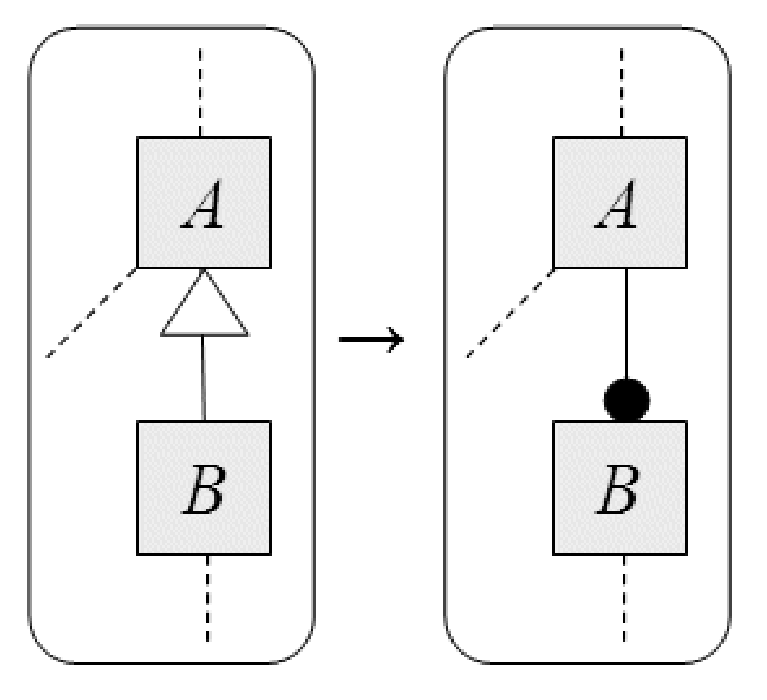
\includegraphics{images/bad-smell1.eps}}
\end{center}
\end{figure}

% template matching
Refactoring designers can apply general FM refactorings based on template matching. 
% templates
Each {\em general refactoring} consists of two {\em templates} (patterns) of FMs, on the left-hand (LHS) and right-hand (RHS) sides.
% quando podemos aplicar o refatoramento
A refactoring can be applied whenever the FM matches the template. A matching is an assignment of all meta-features occurring in the LHS template to concrete values.
% o que n�o e mostrado e igual nos dois modelos
Any element omitted by the templates remains unchanged, thus refactoring templates only show differences between FMs. 
% linhas pontilhadas
Moreover, a dashed line on top of a feature indicates that this feature may have a parent feature. A dashed line below a feature indicates that this feature may have additional subfeatures.

% o outro refactoring
A similar refactoring that converts an \emph{or} relation to a mandatory relation can be proposed. 
% corretude
Both refactorings and the following one can be shown correct using a encoding of FMs~\cite{Gheyi:2006aa} in Alloy~\cite{Jakson:2006aa} or using a Prototype Verification System (PVS)~\cite{Owre:2009aa} theory~\cite{Gheyi:2006aa-2}.

\subsection{Constraint imposing the selection of an alternative}

% 1. intuicao
Sometimes a constraint in the model may impose that a child of an alternative relation must always be selected. This bad smell occurs when a global constraint obligates the selection of an \emph{Alternative Feature} or \emph{Or Feature}.
% 2. porque � um problema?
\Fix{Leopoldo: sera que isto eh um problema quando nao eh uma feature
mandatoria que esta impondo a selecao de uma feature alternativa/or?} Since a child must always be selected, the other children of this relationship can never be selected. Detecting this kind of bad smell might reveal constraints that are inconsistent with the feature model relationships.

% 3. explicar em um exemplo toy
For instance, suppose that we add the constraint $B \Rightarrow D'$ in the feature model of Figure~\ref{fig:fm01}. Since B is a mandatory feature of A, it must be selected. From this fact and the previous constraint added, feature D' must be selected.  Therefore, only D' will be a valid option to the alternative feature D. The feature D'' can never be selected.
% conclusao
This may reveal a symptom of a bad design.
% 4. exemplo real

% 5. refatoramento
Refactoring~\ref{ref:ref2} removes this bad smell by excluding the constraint.

\begin{figure}[ht]
\begin{refine}{\ensuremath{\langle}change alternative constraint\ensuremath{\rangle}}
\label{ref:ref2}
\end{refine}
\begin{center}
\leavevmode
\scalebox{0.4}{
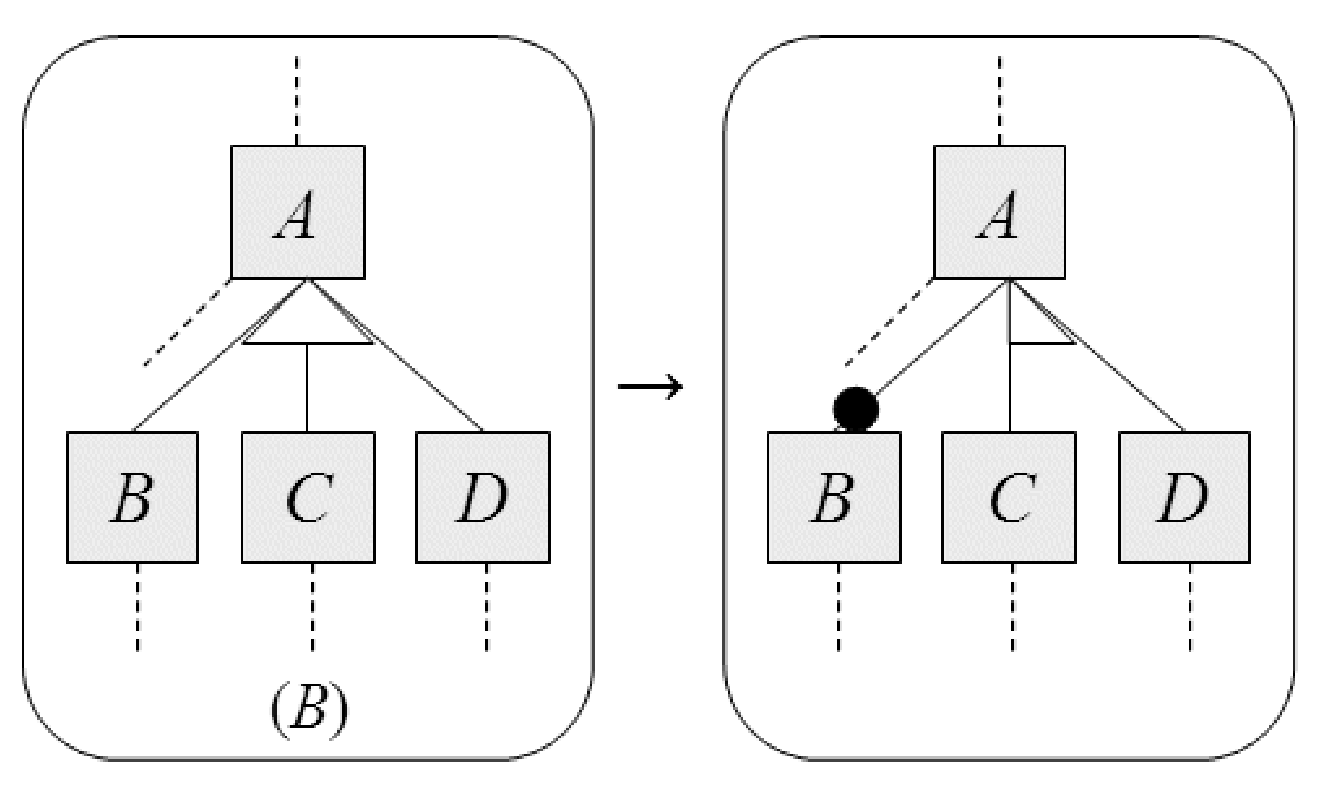
\includegraphics{images/bad-smell2.eps}}
\end{center}
\end{figure}

% refatoramento similar
A similar refactoring can be proposed for an \emph{Or} relationship.
% lei util
In this bad smell and in the following ones, which involve constraints (formulae), we may use Refactoring~\ref{ref:add-formula} in order to prepare the FM to match, for instance, Refactoring~\ref{ref:ref2} template. 
% explicando variavel
The \emph{fs} variable denotes a set of features.
% voltando ao exemplo
In the Figure~\ref{fig:fm01} feature model example, Refactoring~\ref{ref:add-formula} is used to deduce the constraint \emph{D'}. After that, we can apply Refactoring~\ref{ref:ref2}.

\begin{figure}[ht]
\begin{refine}{\ensuremath{\langle}add deducible formula\ensuremath{\rangle}}
\label{ref:add-formula}
\end{refine}
\begin{center}
\leavevmode
\scalebox{0.4}{
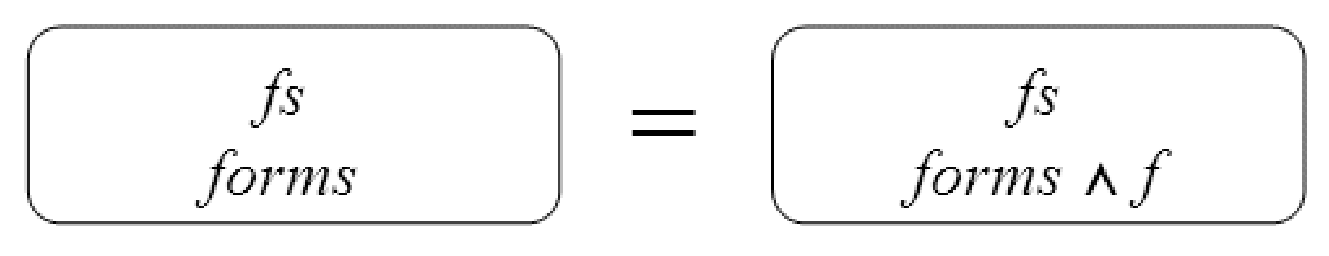
\includegraphics{images/add-formula.eps}}
\end{center}
\noindent ($\leftrightarrow$) \emph{f} can be deduced from \emph{forms} and \emph{fs}. \\
\end{figure}

\subsection{Constraint changing the semantics of a relationship}

% 1. intuicao
Sometimes a feature model may have a constraint making the semantics of a relationship more restrictive. 
% 2. porque � um problema?
This may waste time of domain analysts when understanding the model. It is better to change the relationship. It is easier to understand a model if we include most constraints in the graphical notation.
% 3. explicar em um exemplo toy
One example of this bad smell is present in the feature model of Figure~\ref{fig:fm01}.
As we explained in Section~\ref{sec:intro}, in the presence of the global constraint $B \Rightarrow D$, the optional relationship between the features A and D is changed to mandatory. Detecting this kind of bad smell reveals either an improper constraint or an inadequate feature model relationship.
% 4. exemplo real

% 5. refatoramento
This bad smell can be removed by applying Refactoring~\ref{ref:ref3}, which changes from the optional relationship to the mandatory relationship.

\begin{figure}[ht]
\begin{refine}{\ensuremath{\langle}replace optional to mandatory\ensuremath{\rangle}}
\label{ref:ref3}
\end{refine}
\begin{center}
\leavevmode
\scalebox{0.4}{
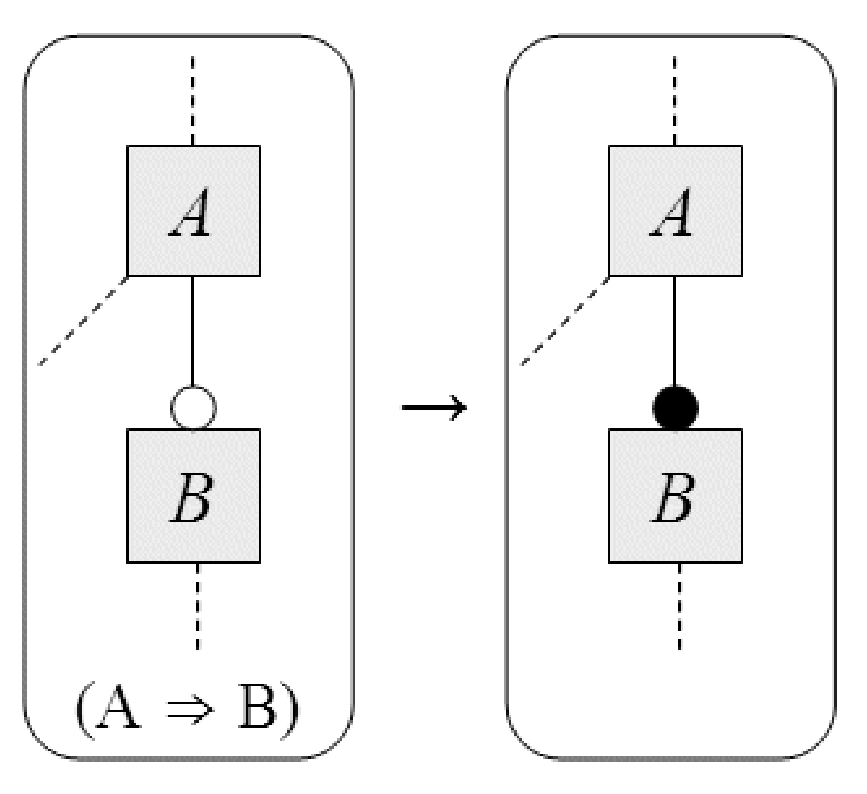
\includegraphics{images/bad-smell3.eps}}
\end{center}
\end{figure}

The same bad smell can appear between other relationships. For example, sometimes we can convert an \emph{Or} relationship to an \emph{Alternative} relationship. A number of refactorings can be useful for removing them~\cite{Gheyi:2009aa}.

\subsection{Redundant constraints}

% 1. intuicao
It is useful to add redundant constraints in order to make the model easier to understand. A redundant constraint does not narrow the number of instances (configurations) of a feature model --- so, it does not define any additional restriction to the feature model. The number of valid configurations is the same.
% 2. porque � um problema?
However, sometimes when we add a number of redundant constraints, it may be difficult for domain analysts to understand the entire model. They may waste time reading some constraints that does not add value to the model. So, in these situations, it may be better to remove them.

% 3. explicar em um exemplo toy
For example, suppose that one defines a constraint $C \Rightarrow B$ in the feature model of Figure~\ref{fig:fm01}, instead of writing a proper constraint. Note that such a constraint is redundant, since feature B must be present in any valid configuration of this feature model. 
% conclusao
Therefore, detecting this kind of bad smell might reveal a constraint that was not well specified. 
% 4. exemplo real
% 5. refatoramento
This bad smell can be removed by applying Refactoring~\ref{ref:add-formula} from right to left.

\subsection{Dead features}

% 1. intuicao
This bad smell occurs when a feature, due to a global constraint, could never be selected in the valid instances of a feature model~\cite{Trindad:2006aa}. It may happen because of the number of constraints in the model that may make the model difficult to understand, hence suitable for introducing errors.
% 2. porque � um problema?
This may be a symptom of a bad design. 

% 3. explicar em um exemplo toy
For instance, if the constraint $B \Rightarrow \neg C $ is added to the feature model of Figure~\ref{fig:fm01}, the feature C becomes a dead feature. It will never be present in any configuration of the feature model. 
% conclusao
If a feature is dead, it may be useless to the model and should be removed from it, or it may reveal a problem in the model (overconstrained) and we should remove some constraints.

% 4. exemplo real
% 5. refatoramento
Two refactorings can be used to remove this bad smell. Refactoring~\ref{ref:remove-formula} can be used to remove some constraints in the overconstrained model. 

\begin{figure}[ht]
\begin{refine}{\ensuremath{\langle}remove formula\ensuremath{\rangle}}
\label{ref:remove-formula}
\end{refine}
\begin{center}
\leavevmode
\scalebox{0.4}{
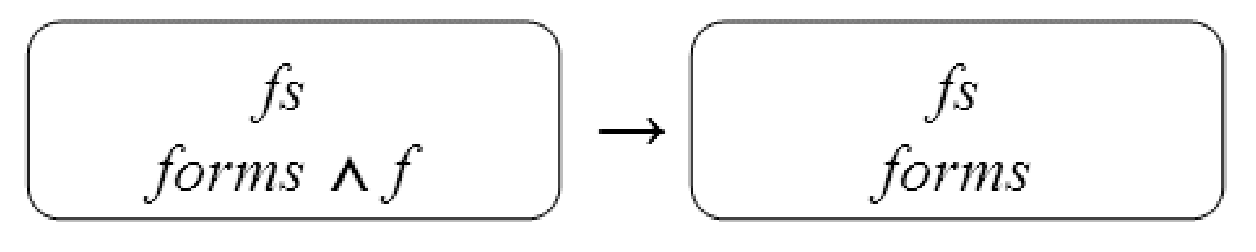
\includegraphics{images/remove-formula.eps}}
\end{center}
\end{figure}

In case the feature must be removed, we can apply Refactoring~\ref{ref:remove-feature}. We remove it from the model, and replace its occurrence in all constraints by \emph{false}.

\begin{figure}[ht]
\begin{refine}{\ensuremath{\langle}remove dead feature\ensuremath{\rangle}}
\label{ref:remove-feature}
\end{refine}
\begin{center}
\leavevmode
\scalebox{0.4}{
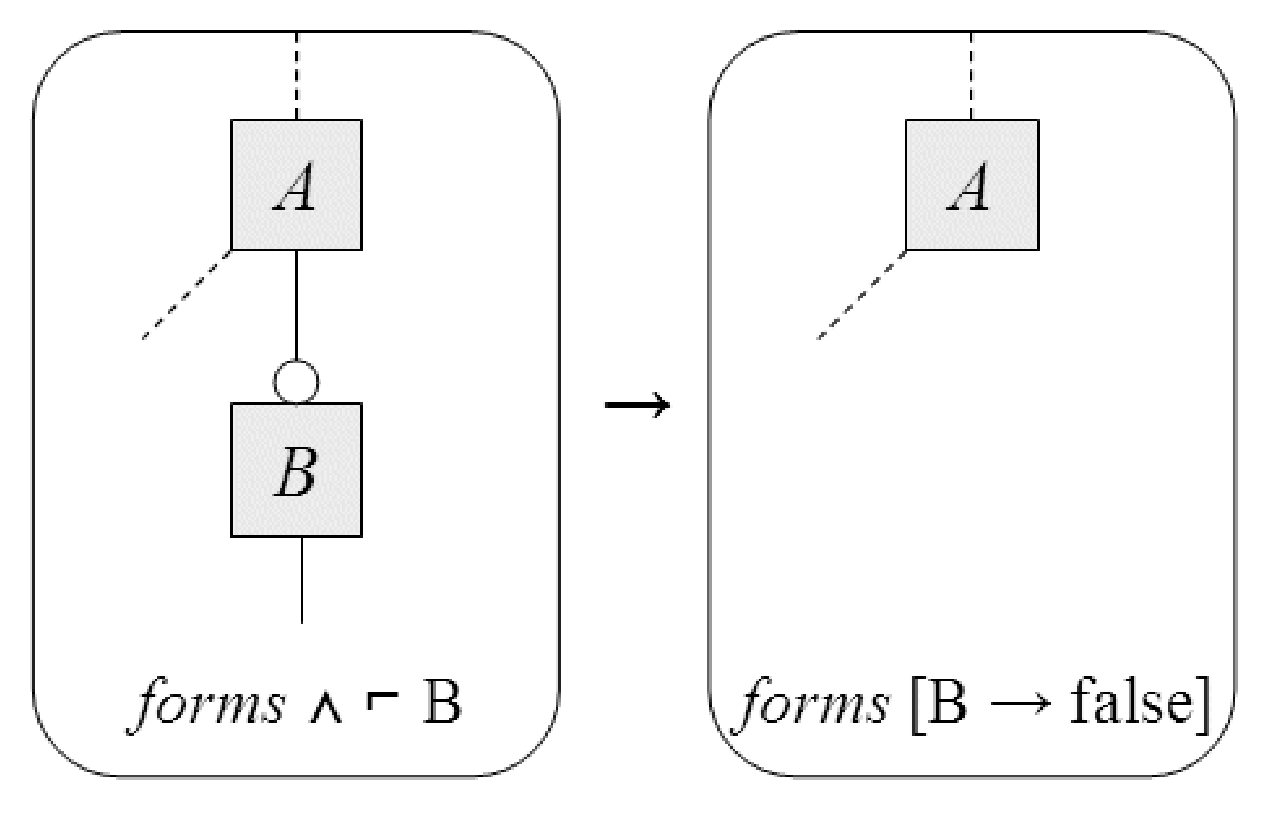
\includegraphics{images/remove-feature.eps}}
\end{center}
\end{figure}

\subsection{Inconsistent Model}

% 1. intuicao
This bad smell occurs when a feature model does not have any valid
configuration due to contradicting constraints. It may happen when
overconstraining the model, making it difficult to understand, hence, suitable
for introducing errors.
% 2. porque � um problema?
In general, this may be a symptom of a bad design and an error. 

% 3. explicar em um exemplo toy
For instance, if the constraint $C \Rightarrow \neg D $ is added to the feature
model of Figure~\ref{fig:fm01}, the model becomes inconsistent. The feature D
must always be selected.
% conclusao
If a model does not have a valid configuration, it may reveal an error in the
model design. In general, it is useless to have an inconsistent model.

% 4. exemplo real
% 5. refatoramento
In order to remove the contradiction, we first use a tool, such as proposed by Benavides~\cite{Trinidad:2008aa-2}, which extracts the minimum set of constraints that make the model inconsistent. After debugging the model, the domain analyst should check which set of constraints must be removed. Then, we can apply Refactoring~\ref{ref:remove-formula} to remove them from the model.



\section{Tool Support}\label{sec:tool-support}

We have developed a Haskell library and a set of tools for checking errors and bad smells in feature models. Therefore, offering these asserts to the Haskell community is another contribution of this work--- since, to our knowledge, there is no corresponding set of libraries and tools developed in functional languages. In short, these libraries and tools make available:

\begin{itemize}
 \item data types for feature modeling in Haskell;
 \item functions for checking if a feature model is well typed;
 \item functions for detecting bad smells in feature models;
 \item functions for checking if a feature model is satisfiable;
 \item functions for checking if a selection of features is a valid instance of a feature model; and
 \item integration with existing tools, such as Feature Modeling Plugin and FeatureIde 
\end{itemize}   

We start this section by presenting a few design decisions regarding the development of the feature model library. Then, we present some analysis of benchmarking that were performed on three distinct feature models available at~\cite{Group:2009yg}: \emph{eShop feature model} (325 features), \emph{Model transformation} (113 features) and \emph{Web portal} (49 features). These feature models have been widely described in the literature. We have also checked the satisfiability functions on models with 1000 features. 

\subsection{Design decisions}

For checking satisfiability, we have implemented two solutions. The first one is a purely functional implementation, using the Funsat Haskell library. Besides informing if a feature model is satisfiable or not, using this approach we can also get a valid instance for the model. However, this library is not optimized for complex feature models. For this reason, we have also developed an interface with the Minisat SAT solver, an open source project developed in C.    

\subsection{Benchmark analysis}

We evaluated our tools in small and medium-sized feature models that are publicly available. Since these models have been widely used in the literature, we believe that they are representative to our analysis. Basically, here we present  that our tools correctly detect errors and bad smells in reasonable time. Some of the existing models that we took already present some kind of error. Most of them are related to duplicated features. Bad smells were introduced in the evaluated feature models. 

For each feature model we evaluated three operations: type checker (TC), satisfiability checker (SC), and bad smells detection (BSD). Additionally, in order to reduce bias, we performed 50 evaluations for each pair \emph{operation and feature model}. We conducted all measurements on the same Mac OS-X with 2.16 GHz and 2 GB of RAM. The time, measured in milliseconds, was collected using the \emph{BenchPress} library~\cite{Tibell:2009rm}. The mean time for each pair is present in Table~\ref{tab:analysis}.

\begin{table}[htdp]
\begin{center}
\begin{tabular}{|l|c|c|c|c|} \hline
Feature model 			& Features 			& TC 	& SC 	& BSD      		\\ \hline
Web portal       			& 49                             	& 4.8 	& 4.5 	& 125.78 		\\ \hline
Model transformation       & 113			    	& 4.5	& 20.70	& 1339.03		\\ \hline 
eShop				& 325				& 15.27  	& 125.76	& 25806.05 	\\ \hline
\end{tabular}
\end{center}
\caption{Benchmark results}
\label{tab:analysis}
\end{table}

We can observe that the time required for detecting bad smells increases significantly as the number of features increase. For instance, checking bad smells in the \emph{eShop} feature model took approximately 25 seconds. This number is almost 20 times greater than the time required for detecting bad smells in the \emph{Model transformation} feature model. However, we claim that even in this case, the response time is reasonable, since it might significantly reduce the effort for detecting bad design decisions manually. Additionally, the current implementations of the corresponding functions were developed without considering performance. For instance, the function for detecting dead features (Listing~\ref{lst:dead})is extremely time consuming, since, for each optional feature, it makes a call for the satisfiability function. Optimizing these functions is a future activity. 

\begin{lstlisting}[belowskip=12pt,frame=tb,caption={Function for checking dead features.},label=lst:dead]
checkDeadFeatures :: FeatureModel -> [Feature]
checkDeadFeatures fm = 
 let fm' = addImplies fm
 in
  [ f | f <- features fm
  , isOptional f
  , not (isSatisfiable fm' f)
  ]
\end{lstlisting} 







  



  
 



\section{Evaluation}

% Discuss the benefits of applying the DR language in different case studies
% - Health watcher
% - choose one of the cases: TaRGeT, Games, Mobile Media, FLIP, \ldots
% Evaluate the benefits based on metrics
% - Concern metrics or Lattix Metrics

Example 1: Auditing Concern without Design Rules

The auditing concern must be triggered when inserting, removing,
updating, or searching for a complaint.

Two teams working in parallel without design rules: the first one
works on the base code (the ComplaintRepository) and the second one
works on the auditing concern. Such a concern is implemented as an
aspect.

\scriptsize
\begin{lstlisting}[frame=single, caption={Complaint Repository implementation.},label=lst:complaint-repository, language=Java]
public class ComplaintRepository implements IComplaintRepository {

    public int insert(Complaint c) throws RepositoryException, ObjectAlreadyInsertedException {

    }

    public void update(Complaint c) throws RepositoryException, ObjectNotFoundException {

    }

    public void remove(int id) throws RepositoryException, ObjectNotFoundException {

    }

    public Complaint search(int id) throws RepositoryException, ObjectNotFoundException {

    }

}
\end{lstlisting}
\normalsize

Aspect for implementing the auditing concern:

\scriptsize
\begin{lstlisting}[frame=single, caption={Complaint Repository implementation.},label=lst:complaint-repository, language=Java]
public aspect AuditingAspect {

    pointcut auditWhen():
           execution(int ComplaintRepository.insert(Complaint)
        || execution(void ComplaintRepository.update(Complaint)
        || execution(void ComplaintRepository.remove(int)
        || execution(Complaint ComplaintRepository.search(int)

    after() returning(): auditWhen() {
        // audit code.
    }

}
\end{lstlisting}
\normalsize

In the meanwhile, suppose that the teams are working on their
respective concerns (the repository and the auditing concerns). Now,
suppose that the team of the repository changes the following:

\begin{itemize}
    \item the insert method returns void instead of int; and

    \item the remove and search methods should take as parameter the
    Complaint object instead of an id.
\end{itemize}

Such changes might break the aspects...

% =================================== at� aqui entraria na se��o 2...

% ===== se��o 4

Design Rule:

\scriptsize
\begin{lstlisting}[frame=single, caption={Complaint Repository implementation.},label=lst:complaint-repository, language=Java]
dr AuditingDesignRule {

    class ComplaintRepository {

        public int insert(Complaint c) throws RepositoryException, ObjectAlreadyInsertedException {}

        public void update(Complaint c) throws RepositoryException, ObjectNotFoundException {}

        public void remove(int id) throws RepositoryException, ObjectNotFoundException {}

        public Complaint search(int id) throws RepositoryException, ObjectNotFoundException {}

    }

    aspect AuditingAspect {

        pointcut auditWhen():
            execution(int ComplaintRepository.insert(Complaint)
            || execution(void ComplaintRepository.update(Complaint)
            || execution(void ComplaintRepository.remove(int)
            || execution(Complaint ComplaintRepository.search(int)

        % precisa do args aqui...??? Acho que sim...

        after() returning(): auditWhen() {
            xcall(void Auditing.auditComplaint(Complaint));
        }

    }

}
\end{lstlisting}
\normalsize

XPI of this example:

public aspect AuditingXPI {

    pointcut auditWhen():
        execution(int ComplaintRepository.insert(Complaint)
        || execution(void ComplaintRepository.update(Complaint)
        || execution(void ComplaintRepository.remove(int)
        || execution(Complaint ComplaintRepository.search(int)

    pointcut callToAudit(): call(void Auditing.auditComplaint(Complaint));

    declare error: (callToAudit() && !within(AuditingXPI)):
        "Contract violation: the auditComplaint method can not
        be called outside the aspect AuditingXPI";

}

In order to guarantee the contract that classes, aspects and their
respective methods and advices must exist, we can informally
document it like a prose, as mentioned in~\cite{}. Obviously, in
this case the contract is not verified by using the AspectJ
compiler, for instance.

However, we can guarantee the aforementioned contract by using
Aspect-Aware interfaces~\cite{}. Figure TAL illustrates that when a
pointcut does not match any piece of code, the compiler emits a
warning to the developer. Such a warning might be used to alert the
developer that some method must exist, for example.

\section{Related work}

% Compare our work with relevant ones
% - open modules
% - XPIs
% ..
% We conclude that we should improve this section


\section{Concluding Remarks}

% a summary of the main concluding remarks 
% of the paper.




% An example of a floating figure using the graphicx package.
% Note that \label must occur AFTER (or within) \caption.
% For figures, \caption should occur after the \includegraphics.
% Note that IEEEtran v1.7 and later has special internal code that
% is designed to preserve the operation of \label within \caption
% even when the captionsoff option is in effect. However, because
% of issues like this, it may be the safest practice to put all your
% \label just after \caption rather than within \caption{}.
%
% Reminder: the "draftcls" or "draftclsnofoot", not "draft", class
% option should be used if it is desired that the figures are to be
% displayed while in draft mode.
%
%\begin{figure}[!t]
%\centering
%\includegraphics[width=2.5in]{myfigure}
% where an .eps filename suffix will be assumed under latex, 
% and a .pdf suffix will be assumed for pdflatex; or what has been declared
% via \DeclareGraphicsExtensions.
%\caption{Simulation Results}
%\label{fig_sim}
%\end{figure}

% Note that IEEE typically puts floats only at the top, even when this
% results in a large percentage of a column being occupied by floats.


% An example of a double column floating figure using two subfigures.
% (The subfig.sty package must be loaded for this to work.)
% The subfigure \label commands are set within each subfloat command, the
% \label for the overall figure must come after \caption.
% \hfil must be used as a separator to get equal spacing.
% The subfigure.sty package works much the same way, except \subfigure is
% used instead of \subfloat.
%
%\begin{figure*}[!t]
%\centerline{\subfloat[Case I]\includegraphics[width=2.5in]{subfigcase1}%
%\label{fig_first_case}}
%\hfil
%\subfloat[Case II]{\includegraphics[width=2.5in]{subfigcase2}%
%\label{fig_second_case}}}
%\caption{Simulation results}
%\label{fig_sim}
%\end{figure*}
%
% Note that often IEEE papers with subfigures do not employ subfigure
% captions (using the optional argument to \subfloat), but instead will
% reference/describe all of them (a), (b), etc., within the main caption.


% An example of a floating table. Note that, for IEEE style tables, the 
% \caption command should come BEFORE the table. Table text will default to
% \footnotesize as IEEE normally uses this smaller font for tables.
% The \label must come after \caption as always.
%
%\begin{table}[!t]
%% increase table row spacing, adjust to taste
%\renewcommand{\arraystretch}{1.3}
% if using array.sty, it might be a good idea to tweak the value of
% \extrarowheight as needed to properly center the text within the cells
%\caption{An Example of a Table}
%\label{table_example}
%\centering
%% Some packages, such as MDW tools, offer better commands for making tables
%% than the plain LaTeX2e tabular which is used here.
%\begin{tabular}{|c||c|}
%\hline
%One & Two\\
%\hline
%Three & Four\\
%\hline
%\end{tabular}
%\end{table}


% Note that IEEE does not put floats in the very first column - or typically
% anywhere on the first page for that matter. Also, in-text middle ("here")
% positioning is not used. Most IEEE journals/conferences use top floats
% exclusively. Note that, LaTeX2e, unlike IEEE journals/conferences, places
% footnotes above bottom floats. This can be corrected via the \fnbelowfloat
% command of the stfloats package.

% use section* for acknowledgement
\section*{Acknowledgment}

The authors would like to thank...more thanks here


% trigger a \newpage just before the given reference
% number - used to balance the columns on the last page
% adjust value as needed - may need to be readjusted if
% the document is modified later
%\IEEEtriggeratref{8}
% The "triggered" command can be changed if desired:
%\IEEEtriggercmd{\enlargethispage{-5in}}

% references section

\bibliographystyle{abbrv}
\bibliography{splc2009}






% that's all folks
\end{document}


